%\documentclass[11pt, oneside]{article}   	
%\usepackage{geometry}    
%\geometry{letterpaper}                 		
\input preamble.tex
\newcommand{\ig}[2][width=4in]{\includegraphics[#1]{#2}}    		
\usepackage{graphicx}					
\usepackage{amssymb}
\usepackage{pgfplotstable}
\usepackage{float}
\usepackage{caption}
\captionsetup[table]{justification=justified,singlelinecheck=false, position=bottom}
\begin{document}

\header {\today}							
\title{Rutherford Scattering}
\author{Ekta Patel \& Brandon Booth-Dunbar}

\section{Abstract}
\begin{em} In this lab, we verify the Rutherford formula for nuclear scattering. The distribution of alpha particles scattered by gold foil can be observed as a function of the scattering angle, which relies on the distance between the foil and a detector. The theory behind the formula was originally developed in 1913 by Ernest Rutherford and his students. \end {em}

\section{Theory}
%B&E
Geiger and Marsden formed the first preliminary theory for the Rutherford model of the atom. They were able to gather that most $\alpha$-particles, He nuclei, passed right through a thin foil without being deflected. However, there were many particles that experienced large angle scattering. Rutherford was able to show that a positively charged nucleus has a differential scattering cross-section for charged particles that is given by:
\begin {equation} \frac{d\sigma}{d\Omega}(\theta)= \frac{Z^2z^2e^4}{16E^2} \frac{1}{sin^4(\theta/2)}\end{equation} where $Ze$ is nuclear charge, $ze$ is charge of the scattered particle and $E$ is the energy of the scattered particle. $\theta$ is the scattering angle that we determine to be a function of a length, $Y$ that is varied between the foil and the detector.\\
\newline The rate of detected particles, $N_2$, can be expressed in terms of $N_0$, the total number of particles emitted by the source per unit solid angle. Using the geometry of the set up and the Rutherford formula, the rate of detected particles is determined by the following formula:

\begin{equation} N_2= N_0\times G\times f(Y) \end{equation}
\begin{equation} N_2=N_0\times \left( \frac{nA_2Z^2z^2e^4}{R_1^2r_1^2 16 E^2}\right)\times \left(\frac{cos\theta_2 sin\theta_2^2}{sin(\theta/2)^4}\right) \end {equation}
Solving the equation for $f(Y)$ so that we can plot $Y$ vs. $f(Y)$ for a range of 0 cm to 20 cm gives a preliminary idea of how our data should look:
\begin{equation} f(Y)=\frac{cos\theta_2 sin\theta_2^2}{sin(\theta/2)^4} \end{equation} where
\begin{equation} \theta_1=tan^{-1}\left(\frac{r_1}{X}\right)\end{equation} and
\begin{equation} \theta_2=tan^{-1}\left(\frac{r_1}{Y}\right)\end{equation} and
\begin{equation} cos\theta_2=\frac{Y}{\sqrt{Y^2+r_1^2}} \end{equation} and
\begin{equation} sin\theta_2^2=\frac{r_1^2}{Y^2+r_1^2}, \end{equation} therefore:
\begin{equation} f(Y)= \frac{\frac{Y}{\sqrt{Y^2+r_1^2}} \frac{r_1^2}{Y^2+r_1^2}}{sin(0.5(tan^{-1}\left(\frac{r_1}{X}\right) + tan^{-1}\left(\frac{r_1}{Y}))\right)^4.} \end{equation}\\
Plotting this function for f(Y) over an interval of 0 to 20cm, we have:

\begin{figure}[h!]
\begin{center}
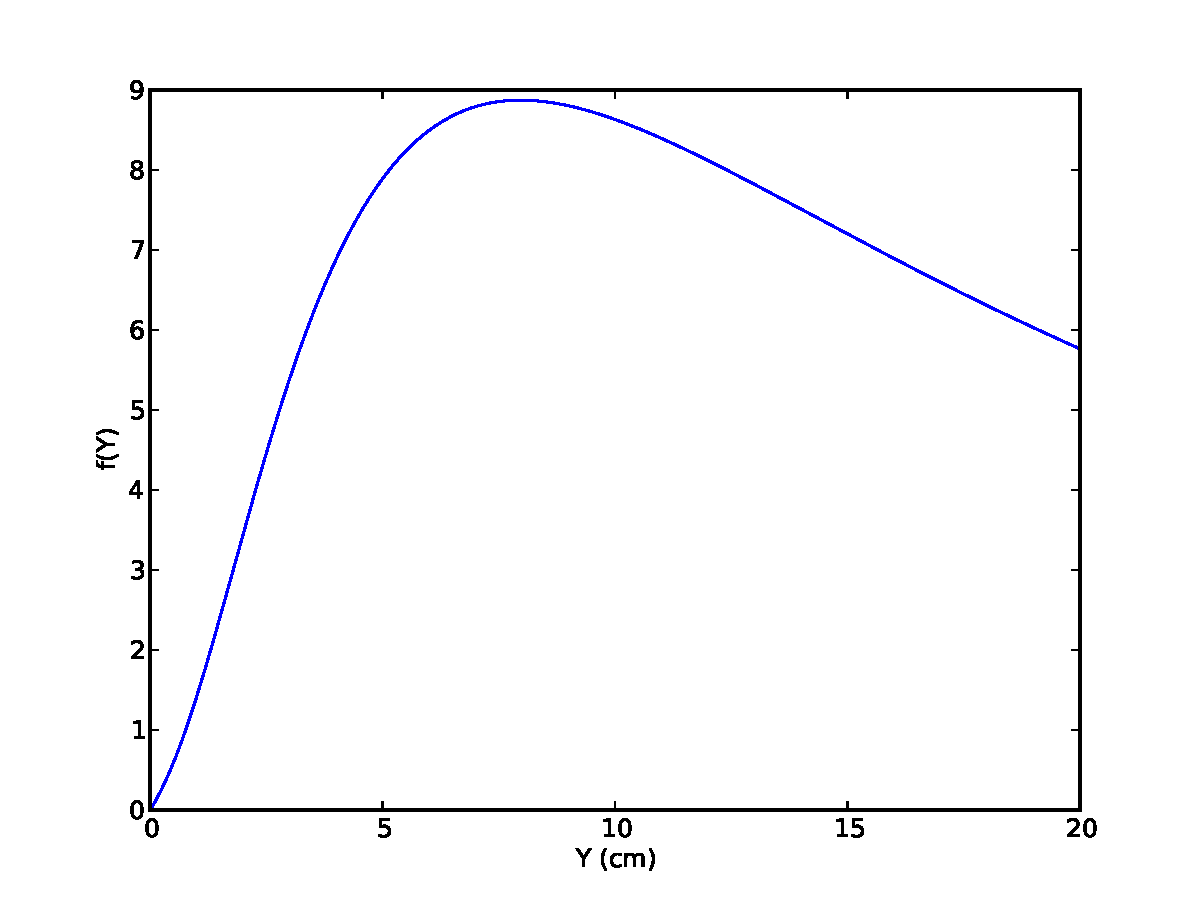
\includegraphics[width=4in]{preliminary_plot.pdf}
\caption{The theoretical values for the third term in the rate of detected particles($N_2$) that varies with the scattering angle as a function of length.}
\end{center}
\end{figure}

\section{Experimental Methods}
\subsection{Apparatus}
\subsection{Procedures}
\subsection{Calibration}
\subsection{Recording Data}


\section{Results and Discussion}
%Ekta

\section{Conclusion}
%Brandon


\begin{thebibliography}{99}
\bibitem{electron}Sleator, Tycho, and Windt, David, \begin{em}Rutherford Scattering. \end{em}Experimental Physics. V85.0112. Spring, 2011.
\end{thebibliography}
\end{document}
